\section*{Executive Summary}
\addcontentsline{toc}{section}{Executive Summary}

Data Challenge 2 (DC2) is the second in a series of prototypes of the LSST Data Management System (DMS).  Through these data challenges, we seek to identify the most challenging technical problems to building a DMS that meets the LSST science goals.  We prototype specific solutions to these challenges with the expectation that by the start of the construction phase of the telescope, we will have a well-defined plan for how to build a DMS that can perform at the level needed by first light.  Despite the prototyping nature of the data challenges, we are not producing throw-away code; rather, we expect that the software we produce in the data challenges will serve as the foundation for the DMS that will be completed during the construction phase.

\subsubsection*{Results}

In Data Challenge 1 (DC1), we focused on the DMS middleware design for supporting nightly processing.  In particular, we designed and prototyped the pipeline framework that would host the scientific algorithms used to process the data coming from the telescope.  DC1 did not include actual implementations of scientific algorithms but rather tunable \textit{resource consumers} that simulate the expected computation load of the algorithms.

In DC2, we focused on replacing these simulators with real implementations of the scientific algorithms.  More of our software architecture was refined, including the choice of using C++ to implement compute-intensive components and Python for integrating components, and we built a software development environment.  Consequently, we updated the pipeline framework into this new architecture.  We executed our second-generation nightly pipeline on real astronomical data from the Canada-France-Hawaii Telescope's Legacy Survey.

In all, we developed 49000 lines of C++ in 205 classes and 2330 methods, and 34000 lines of Python in 387 classes and 2111 methods.  The effort was 9 FTE for a year.  This is well above the productivity needed for MREFC development, allowing for increased levels of testing and more stringent performance needed for the production system.

\subsubsection*{Applications}

We developed, unit tested, and executed Image Subtraction, Detection, Moving Object Processing, and Association Pipelines.  All of the pipelines were developed as ``pluggable'' Stages within the Pipeline Harness and used the newly-developed Event system to synchronize.

We executed over 100 runs of the pipelines at various levels of completeness, including several runs at ``full'' scale, i.e.~with all of the processing nodes available. These runs were executed on a small dedicated cluster hosted at NCSA. We have focused our analysis of the results on three particular runs that featured identical versions of the software: \code{rlp0127}, \code{rlp0128}, and \code{rlp0130}.  In these runs, the Image Processing and Detection (IPD) pipeline featured 1 master pipeline process and 36 slice process running across six nodes of the cluster.  The Moving Objects Prediction System (MOPS) pipeline ran on one node with 3 slice processes.  The Association pipeline ran entirely in one process, the master process, on the node where the database was located.

Each of these runs operated on a different set of 36 amplifier-sized images from the same set of mosaic CFHT-LS D4 exposures (amplifier numbers 73--108, 37--72, and 181--214, respectively).  From a total of 288 possible amplifier images per exposure, the amplifier sets were chosen to sample different areas of the focalplane; \Fig{SumFigMegaCamMap} illustrates the location of these amplifier sets.  The number of visits completed in each run were 53, 62, and 62, respectively, for a total of 177 visits.   A summary of the three runs, including the number of images successfully processed, appears in \Table{TSum-1}.  

\begin{figure}[htbp]
\begin{center}
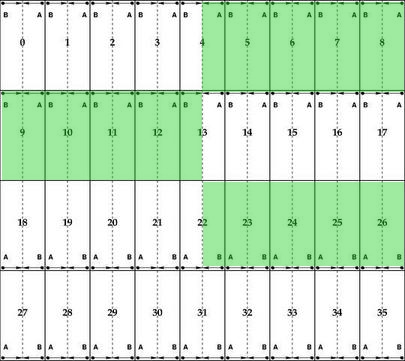
\includegraphics[height=60mm] {figures/MegaCamMap}
\caption{Map of the CFHT MegaCam focalplane.  The area covered by DC2
  runs rlp0127, rlp0128, and rlp0130 are shaded.}
\label{SumFigMegaCamMap}
\end{center}
\end{figure}

\begin{table}[htbp]
\begin{center}
\caption{Summary of DC2 Reference Runs\label{TSum-1}}
\vspace{\baselineskip}
\begin{tabular}{ | r | r | r | c | r | r | r |}
\hline
runId & nVisits & nAmps & Amp IDs & inputImages & outputImages & outputFrac \\ \hline
rlp0127 & 53 &  36 &  73-108 & 1908 & 1875 & 0.983 \\ \hline
rlp0128 & 62 &  36 &  37-72  & 2232 & 2228 & 0.998  \\ \hline
rlp0130 & 62 &  36 & 181-214 & 2232 & 2213 & 0.991 \\ \hline
Total   & --- & 108 &   ---    & 6372 & 6316 & 0.991 \\ \hline
%\hline
\end{tabular}
\end{center}
\end{table}

We note that the DC2 pipeline will run without modification on much larger clusters.  A cluster with 288 cores would allow the full CFHT MegaCam mosaic to be processed in parallel.  We expect such hardware to be available to us very soon, and we will supplement this report with results from such runs when they are available.  We discuss scalability implications for LSST later.

All of these applications extensively reused the object-oriented Application Framework that was developed in DC2. This Framework was designed to standardize astronomical data representations and core functions so that they can be reused in any pipeline.

The goals for the application framework and for the algorithms implemented using it have been nearly completely achieved, and this is clearly one of the major results of DC2.  The prototype nightly processing pipelines include the required algorithms, and have worked reliably as measured by the fraction of input images that are successfully processed through the pipeline.

The one application goal we have not yet achieved is establishing a realistic object/source database for use by the broader collaboration. While we have successfully implemented the database to the schema as designed, and populated it with properly structured and linked data, the data quality is not yet sufficient to be useful to the broader collaboration.  The reasons for this are well understood and described in this report, and much of the application code required to achieve the goal has already been written and tested.  We anticipate achieving this goal fully in the course of Data Challenge 3.

\subsubsection*{Middleware and Infrastructure}

Standard middleware was provided for deploying processing to parallel nodes in a cluster, scheduling the processes, inter-process communication and data transfer, synchronization via events, and for saving data to and retrieving data from FITS files, serialized object files, and relational databases.

The innovation of the newly implemented pipeline harness is in the way it effectively balances to use of Python and C++.  Application Stages --- the container for the scientific algorithms --- can be written with ease in Python.  These stage implementations themselves can be thin wrappers around our C++ classes.  Similarly, the pipeline harness itself is a wrapper around a C++ implementation where the MPI control calls are executed.  Our timing results show that the overhead added to the total processing time by the pipeline harness is very small compared to application processing time.  In particular, the overhead scales linearly with the number of stages ($< 0.1$ seconds per stage) in the absense of event processing.  Sending and receiving events adds additional but still small overhead.  

Our pipeline harness does have a disadvantage that becomes apparent when run on a heterogeneous cluster as we did.  Because of the way we synchronize our processing, the overall speed of the pipeline is limited by the performance of the slowest node.  This is important to consider for the production system.  When we scale up to hundreds or even thousands of cores and run nearly 24 hours a day, one or two defective nodes could easily limit the performance of the entire cluster.  In future data challenges, we will look at strategies for not only minimizing this effect, but also detecting when defective nodes are having a major impact on performance.

\subsubsection*{Development Environment}

We have been quite successful in assembling and configuring an effective software development environment that not only builds the software via a few simple commands but also manages all of the package dependencies.  The ability to have multiple versions of a package simultaneously, as provided by the EUPS system, has been a very powerful feature, particularly during the integration phase when many changes were coming in rapidly.  

Our package distribution system has also been an important mechanism for our distributed team to keep up with the latest changes.  However, the distribution system has suffered from two problems.

First, it has been difficult to ensure smooth installation of third party packages across all of our development platforms.  While the differences between the Mac and Linux platforms have been the most challenging, supporting different distributions of Linux (particularly 64-bit Linux) has not been without problems.

The second problem stems from the amount of time it takes to install a full software stack (as we build everything from source).  This is not only a barrier to new developers but to those of us who maintain the build and distribution system as it makes debugging platform-dependent problems a slow process.  We hope our future experiments with virtual machines will alleviate the barrier for new developers.  

\subsubsection*{Required software developments for DC3}

As we prepare to transition from the completion of DC2 to the development of DC3, it is appropriate to assess what improvements will be required in the existing LSST software.  First, we emphasize that our experience with the DC2 framework, and with the software development system with which it was designed, built, and documented, has been very positive.  We will use it as the foundation for DC3.

As we fully expected, however, we will need to extend it in various ways. The preceding sections of this report have identified a number of detailed improvements to the existing framework classes that we expect to need for DC3.  We will not recap those here, rather taking a somewhat higher level view.  The main required developments that we have identified are:

\begin{itemize}

\item We need to define the role of the middleware orchestration layer in catching exceptions and possibly mediating adaptive behavior of the pipeline stages in recovering from problems such as algorithmic failures.

\item We need to define API and mechanism for inter-slice communication (neither present nor required for DC2).  We have at least three usecases that require some form of inter-slice communication: cross-talk correction; the association pipeline (which is currently using shared memory outside of the pipeline framework for this), and handling Footprints that cross amplifier boundaries.

\item In a related issue, the LSST focalplane --- with its roughly 3000 amplifiers, 200 ccds, and 21 rafts --- has lots of boundaries. We need to carefully assess where processing needs to take account of what's on the other side of a boundary.

\item We need to address the performance issues with accessing pixels under \code{vw}, as described in the next subsection.  This is the source of our only significant performance problem.

\item We need to further develop the image subtraction software to improve the data quality of the subtracted images.

\end{itemize}

\subsubsection*{Scaling to LSST}

Finally, we need to assess where we stand in relation to the final performance requirements for LSST.  The input images we have used for DC2 have 340 Megapixels, just over 10\% the size of the LSST focalplane.  They also have very similar pixel scale and somewhat greater exposure depth as a single LSST exposure.  Although the hardware available for DC2 prevented us from processing full images in parallel, the DC2 software is designed to do so without modification. We expect to make such runs shortly after completion of this report. We are thus very close to processing a data stream that is 10\% that of LSST.  This is in line with the expectations for DC2 set in the MREFC proposal.

We do have a significant shortfall in the per-node performance on the nightly processing pipeline, achieving about 20\% of what is required to meet the 60 sec alert processing latency.  As discussed above, we believe that we have isolated the performance problem to a small section of code that utilizes the Vision Workbench (\code{vw}) library to access image pixels. Our strategy for verifying that we are on track to achieve the full LSST performance level is to:

\begin{itemize} 

\item Complete the full focalplane DC2 runs, utilizing 288 nodes for the IPD pipeline.  This will verify that the middleware framework is not limiting performance. 

\item Work with the \code{vw} group at NASA Ames to resolve the pixel access performance issues that are limiting image subtraction speed. 

\item In the event that \code{vw} continues to be a performance issue, we will replace it.  The application APIs would not be significantly impacted by such a change, so changes to the existing software stack would be very localized. 

\item As a risk reduction strategy, we will continue our ongoing effort to track and evaluate the performance of GPU and related architectures for image processing tasks.  Based on present application experience, these offer at least a factor of 4 improvement in per-node performance, which gives ample headroom to meet full LSST performance. 

\item We need to address load balancing issues inherent to our pipeline harness to ensure that a few defective nodes in a cluster do not drag down the performance of a massively parallel pipeline.   

\end{itemize}

We will have results from the first three steps in this plan by May, 2008.
